\documentclass[border=3pt,tikz]{standalone}
\usepackage{amsmath}
\usetikzlibrary{arrows.meta}
\usetikzlibrary{calc}
\begin{document}
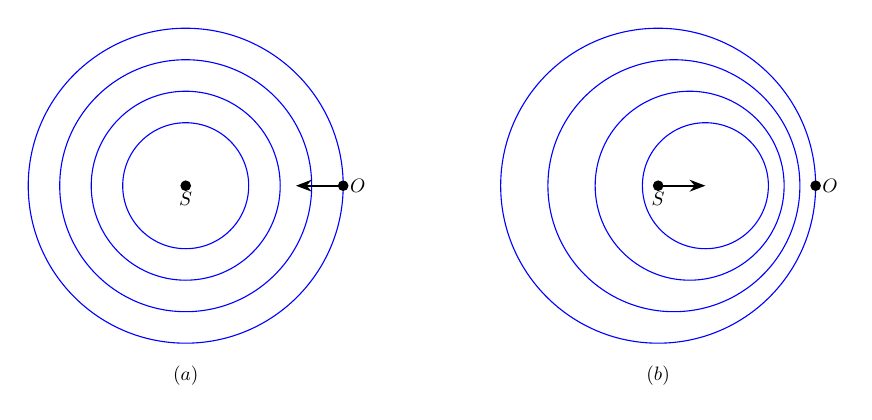
\begin{tikzpicture}[line cap=round, scale = 2]
    % 관찰자가 움직일때의 도플러 효과
    \draw[fill=none, blue](0,0) circle (0.4);
    \draw[fill=none, blue](0,0) circle (0.60);
    \draw[fill=none, blue](0,0) circle (0.80);
    \draw[fill=none, blue](0,0) circle (1);
    
    \filldraw[] (0, 0) circle (0.03) node[below, scale=0.7] {$S$};
    \filldraw[] (1, 0) circle (0.03) node[right, scale=0.7] {$O$};
    \draw[thick, -{Stealth[length=2mm]}] (1, 0) -- (0.7, 0);
    
    \node [below, scale = 0.7] at (0, -1.1) {$(a)$}; 
    
    \begin{scope}[shift={(3,0)}]
    \draw[fill=none, blue](0,0) circle (1);
    \draw[fill=none, blue](0.1,0) circle (0.8);
    \draw[fill=none, blue](0.2,0) circle (0.60);
    \draw[fill=none, blue](0.3,0) circle (0.4);
    
    \filldraw[] (0, 0) circle (0.03) node[below, scale=0.7] {$S$};
    \filldraw[] (1, 0) circle (0.03) node[right, scale=0.7] {$O$};
    \draw[thick, -{Stealth[length=2mm]}] (0, 0) -- (0.3, 0);
    \node [below, scale = 0.7] at (0, -1.1) {$(b)$}; 
    \end{scope}
    \end{tikzpicture}
\end{document}